\documentclass[man]{apa7}
\usepackage{lipsum}
\usepackage[utf8]{vietnam}
\usepackage{csquotes}
\usepackage[style=apa,sortcites=true,sorting=nyt,backend=biber]{biblatex}
\DeclareLanguageMapping{american}{american-apa}
\addbibresource{bibliography.bib}
\usepackage{amsmath, amsfonts, amssymb, amsthm}
\usepackage{indentfirst}
\setlength{\parindent}{0.5in}
\usepackage[left=1in, right=1in]{geometry}

\title{Hàm băm mật mã học}
\shorttitle{HÀM BĂM MẬT MÃ HỌC}
\author{
Nhóm 19.\\
Nguyễn Bá Anh 20203309\\
Nguyễn Thị Vân Anh 20200036\\
Nguyễn Đức Huynh 20206149\\
Nguyễn Lương Quỳnh Trang 20206175\\
Bùi Thanh Tùng 20206181\\[0.5cm]
Viện Toán ứng dụng và Tin học \\
Đại học Bách khoa Hà Nội\\[0.5cm]
Học phần: Mật mã và độ phức tạp thuật toán\\
PGS. TS. Nguyễn Đình Hân\\ 
TS. Ngô Thị Hiền\\[0.5cm]
\today
}
\affiliation{}
% \leftheader{Weiss}
\abstract{Thông tin luôn là một trong những nguồn tài nguyên quan trọng bậc nhất đối với các tổ chức và doanh nghiệp. Với sự phát triển bùng nổ của máy tính và Internet trong thời đại hiện nay, hầu hết thông tin đều được số hóa, vì thế việc truyền đạt chúng trở nên nhanh gọn và thuận tiện hơn bao giờ hết. Tuy nhiên, những thiết bị công nghệ cao ra đời cũng mang theo mối nguy cơ lớn cho vấn đề bảo mật dữ liệu. Để dữ liệu không bị chỉnh sửa, thiệt hại hay bị mất đi, chúng sẽ được mã hóa, để những kẻ tấn công không thể đọc được thông tin trong dữ liệu. Mật mã học ra đời với mục đích nghiên cứu và sử dụng những kĩ thuật, phương thức giao tiếp đảm bảo an toàn thông tin, ngăn chặn bên thứ ba tiếp cận được thông tin.\\ 
\noindent Trong bài báo cáo này, chúng em sẽ trình bày về một khái niệm nền tảng và có ứng dụng đa dạng trong lĩnh vực mật mã học: hàm băm mật mã học. Từ đó, mọi người sẽ có được cái nhìn cơ bản, tổng quan về hàm băm trong mật mã học, bước đầu đánh giá được vai trò của hàm băm, cũng như những ưu thế và rủi ro của nó trong lĩnh vực bảo mật, đồng thời có thể có những sự tìm hiểu và nghiên cứu sâu sắc hơn đối với chủ đề này.\\[0.5cm]
\begin{center}
    \textbf{Lời cảm ơn}
\end{center}
\noindent Trong quá trình hoàn thành bài báo cáo này, chúng em xin trân trọng gửi lời cảm ơn đến PGS. TS.
Nguyễn Đình Hân và TS. Ngô Thị Hiền đã đồng hành cùng chúng em trong bộ môn \textbf{Mật mã và độ phức tạp thuật toán}, sẵn sàng giúp đỡ, tư vấn và giải đáp các vấn đề chúng em đặt ra. Kiến thức trong báo cáo được chúng em tra cứu và tổng hợp phân tích từ nhiều nguồn nên không tránh khỏi có sự sai sót. Vậy nên chúng em hy vọng sẽ nhận được những ý kiến nhận xét từ thầy cô và các bạn để bài báo cáo trở nên hoàn thiện hơn.\\ [0.2cm]
\noindent Chúng em xin chân thành cảm ơn!\\
\noindent \textbf{\textit{Nhóm 19.}}
}

% \keywords{APA style, demonstration}

% \authornote{
   % \addORCIDlink{Daniel A. Weiss}{0000-0000-0000-0000}/

  % Correspondence concerning this article should be addressed to Daniel A. Weiss, Department of Educational Psychology, Counseling and
  % Special Education, A University Somewhere, 123 Main St., Oneonta, NY
  % 13820.  E-mail: daniel.weiss.led@gmail.com}

\begin{document}
\maketitle
\setlength{\leftmargin}{-0.5mm}\tableofcontents
\newpage\,\thispagestyle{empty}

\newpage
\section*{Đóng góp của thành viên}
\setcounter{page}{4}
\noindent Tóm tắt đóng góp của từng thành viên:
\begin{itemize}
    \item Nguyễn Lương Quỳnh Trang: Tìm hiểu và giới thiệu tổng quan về hàm băm mật mã học, chỉnh sửa và hoàn thiện format bài báo cáo theo chuẩn APA
    
    \item Nguyễn Thị Vân Anh: Tìm hiểu và trình bày về tính chất của hàm băm mật mã, chỉnh sửa và hoàn thiện slide trình bày
    
    \item Bùi Thanh Tùng: Tìm hiểu và đưa ra các nội dung chính của báo cáo, tìm hiểu và trình bày về các ứng dụng của thuật toán hàm băm trong lĩnh vực mật mã học
    \item Nguyễn Đức Huynh: Tìm hiểu và trình bày về các phương thức tấn công thuật toán hàm băm, chạy chương trình demo tấn công thuật toán hàm băm
    \item Nguyễn Bá Anh: Tìm hiểu và trình bày về các thuật toán hàm băm, viết chương trình demo thuật toán
\end{itemize}
\noindent Ngoài ra, tất cả các thành viên có đóng góp tích cực trong phân chia công việc, hoàn thành nội dung và nhiệm vụ của mình đúng hạn, tích cực tham gia trao đổi và đóng góp ý kiến cho bài báo cáo chung.\\
\noindent Điểm đánh giá thành viên theo theo chí:
\begin{center}
    \includegraphics[width = 0.98\textwidth]{điểm đánh giá.png}
\end{center}
\addcontentsline{toc}{section}{Đóng góp của thành viên}
\newpage\,\thispagestyle{empty}

\newpage
\section{Giới thiệu về hàm băm trong mật mã học}
\setcounter{page}{5}
\subsection{Khái niệm về Mã khoá đối xứng}
Hệ mật khóa đối xứng (Symmetric Key Cryptography) là một phương pháp mã hóa trong đó cùng một khóa được sử dụng cho cả quá trình mã hóa và giải mã dữ liệu. Đây là một trong những kỹ thuật cơ bản và quan trọng trong lĩnh vực mật mã học, được sử dụng để đảm bảo tính bảo mật và toàn vẹn của thông tin \cite{galil1986symmetric}.
   \begin{figure}[H]
    \centering
    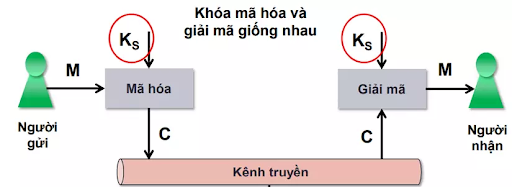
\includegraphics[scale=0.6]{pic/kn_mmdx.png}
    \caption{ Mô hình mã hoá, giải mã bằng khoá đối xứng}
    
\end{figure}
    


\subsection{Ứng dụng của hệ mật khoá đối xứng}
\begin{itemize}
    \item \textbf{Mã hóa dữ liệu}
    \begin{itemize}
        \item  Hệ mật khóa đối xứng được sử dụng để mã hóa dữ liệu lưu trữ trên các thiết bị hoặc cơ sở dữ liệu nhằm bảo vệ thông tin nhạy cảm khỏi truy cập trái phép.
        \item AES (Advanced Encryption Standard) thường được sử dụng để mã hóa dữ liệu trong các hệ thống lưu trữ thông tin quan trọng, như dữ liệu tài chính hoặc y tế.
    \end{itemize}

    \item \textbf{Bảo mật kênh truyền thông}
    \begin{itemize}
        \item  Bảo mật các kênh truyền thông giữa hai hoặc nhiều bên để đảm bảo rằng thông tin truyền tải không bị nghe trộm hoặc thay đổi.
        \item Giao thức SSL/TLS sử dụng mã hóa đối xứng để bảo vệ các kết nối HTTPS, đảm bảo an toàn cho giao dịch ngân hàng trực tuyến, email, và mua sắm trực tuyến.
    \end{itemize}

    \item \textbf{Bảo mật mạng không dây}
    \begin{itemize}
        \item  Mã hóa lưu lượng mạng để bảo vệ dữ liệu truyền qua mạng không dây khỏi bị nghe trộm.
        \item  Các giao thức bảo mật mạng không dây như WPA2 (Wi-Fi Protected Access II) sử dụng mã hóa đối xứng để bảo vệ thông tin truyền qua mạng Wi-Fi.
    \end{itemize}

    \item \textbf{Bảo vệ ổ đĩa và thiết bị lưu trữ}
    \begin{itemize}
        \item  Mã hóa toàn bộ ổ đĩa hoặc thiết bị lưu trữ để bảo vệ dữ liệu nếu thiết bị bị mất hoặc bị đánh cắp.
        \item  BitLocker của Microsoft sử dụng AES để mã hóa toàn bộ ổ đĩa trên hệ điều hành Windows, bảo vệ dữ liệu trong trường hợp mất mát hoặc trộm cắp thiết bị.
    \end{itemize}

    \item \textbf{Bảo mật ứng dụng và dịch vụ đám mây}
    \begin{itemize}
        \item  Mã hóa dữ liệu được lưu trữ và truyền tải qua các dịch vụ đám mây để đảm bảo tính bảo mật và riêng tư của thông tin.
        \item  Các dịch vụ đám mây như Amazon Web Services (AWS) và Google Cloud Platform (GCP) cung cấp các tùy chọn mã hóa đối xứng cho dữ liệu lưu trữ trong đám mây.
    \end{itemize}

    \item \textbf{Mã hóa tin nhắn}
    \begin{itemize}
        \item  Bảo mật tin nhắn trao đổi giữa người dùng qua các ứng dụng nhắn tin tức thời.
        \item  Nhiều ứng dụng nhắn tin như WhatsApp sử dụng mã hóa đầu-cuối (End-to-End Encryption), một dạng mã hóa đối xứng để bảo vệ nội dung tin nhắn khỏi bị đọc trộm.
    \end{itemize}
\end{itemize}
\subsection{Ưu điểm của Hệ mật khóa đối xứng}

\begin{itemize}
    \item \textbf{Tốc độ và hiệu quả}
    \begin{itemize}
        \item  Hệ mật khóa đối xứng sử dụng các thuật toán đơn giản hơn so với hệ mật khóa bất đối xứng, dẫn đến tốc độ mã hóa và giải mã nhanh hơn.
        \item  Điều này làm cho nó phù hợp với các ứng dụng yêu cầu xử lý dữ liệu lớn hoặc yêu cầu thời gian thực, chẳng hạn như mã hóa dữ liệu trên đĩa, truyền thông thời gian thực, và các giao dịch trực tuyến.
    \end{itemize}

    \item \textbf{Đơn giản trong triển khai}
    \begin{itemize}
        \item Các thuật toán mã hóa đối xứng dễ hiểu và dễ triển khai.
        \item Do sự đơn giản của các thuật toán như AES và DES, việc triển khai và tích hợp chúng vào các hệ thống bảo mật dễ dàng hơn. Điều này giúp giảm thiểu lỗi trong quá trình triển khai và duy trì.
    \end{itemize}

    \item \textbf{Tiết kiệm tài nguyên}
    \begin{itemize}
        \item Hệ mật khóa đối xứng tiêu thụ ít tài nguyên hệ thống hơn so với hệ mật khóa bất đối xứng.
        \item  Do tính chất đơn giản của các thuật toán, chúng tiêu thụ ít CPU và bộ nhớ hơn, làm cho nó trở thành lựa chọn lý tưởng cho các thiết bị có tài nguyên hạn chế như điện thoại di động, thiết bị IoT, và các hệ thống nhúng.
    \end{itemize}

    \item \textbf{Bảo mật dữ liệu Tốt}
    \begin{itemize}
        \item Khi được sử dụng đúng cách với một khóa đủ mạnh và bảo mật, hệ mật khóa đối xứng cung cấp mức độ bảo mật rất cao.
        \item  Các thuật toán như AES hiện tại được coi là rất an toàn và chưa có phương pháp tấn công hiệu quả nào có thể phá vỡ chúng trong thời gian hợp lý, nếu khóa được bảo mật tốt.\cite{agrawal2012comparative}
    \end{itemize}

    \item \textbf{Khả năng Tương thích}
    \begin{itemize}
        \item  Hệ mật khóa đối xứng tương thích tốt với nhiều giao thức và tiêu chuẩn bảo mật hiện tại.
        \item  Nó được tích hợp vào nhiều giao thức bảo mật như SSL/TLS cho bảo mật web, IPsec cho mạng, và WPA2 cho mạng không dây, làm cho nó dễ dàng tích hợp vào các hệ thống hiện có.
    \end{itemize}
\end{itemize}

\subsection{ Mặt hạn chế của hệ mật khoá đối xứng}
\begin{itemize}
    \item \textbf{Phân phối khóa}
    \begin{itemize}
        \item  Để hệ mật khóa đối xứng hoạt động, cả người gửi và người nhận phải có cùng một khóa mật. Việc phân phối khóa này phải được thực hiện qua một kênh an toàn, nếu không khóa có thể bị đánh cắp.
        \item Quá trình trao đổi khóa an toàn là một thách thức lớn, đặc biệt trong các mạng lớn hoặc các hệ thống với nhiều người dùng \cite{alenezi2020symmetric}.
    \end{itemize}

    \item \textbf{Quản lý khóa}
    \begin{itemize}
        \item Trong một hệ thống có nhiều người dùng, số lượng khóa cần quản lý tăng lên rất nhanh, do mỗi cặp người dùng cần có một khóa riêng biệt.
        \item  Với \( n \) người dùng, số lượng khóa cần quản lý là \( \frac{n(n-1)}{2} \), điều này dẫn đến sự phức tạp và khó khăn trong việc lưu trữ và quản lý khóa an toàn.
    \end{itemize}

    \item \textbf{Không hỗ trợ xác thực}
    \begin{itemize}
        \item  Hệ mật khóa đối xứng không hỗ trợ cơ chế xác thực nguồn gốc của thông tin.
        \item Vì cả hai bên đều sử dụng cùng một khóa, không có cách nào để xác minh ai là người thực hiện quá trình mã hóa. Điều này làm cho việc xác thực và đảm bảo tính toàn vẹn của thông tin trở nên khó khăn.
    \end{itemize}

    \item \textbf{Không bảo mật trước các cuộc tấn công nhân bản}
    \begin{itemize}
        \item Nếu khóa mật bị đánh cắp, kẻ tấn công có thể mã hóa và giải mã thông tin, gây nguy hiểm cho toàn bộ hệ thống.
        \item Một khi khóa bị lộ, tất cả các thông tin đã mã hóa bằng khóa đó có thể bị giải mã, dẫn đến mất mát dữ liệu và vi phạm an ninh.
    \end{itemize}

    \item \textbf{Thiếu linh hoạt so với hệ mật khóa bất đối xứng}
    \begin{itemize}
        \item Hệ mật khóa đối xứng không linh hoạt bằng Hệ mật khóa bất đối xứng (Asymmetric Key Cryptography).
        \item Hệ mật khóa bất đối xứng sử dụng một cặp khóa công khai và khóa riêng, giúp giải quyết nhiều vấn đề phân phối khóa và xác thực, mặc dù có tốc độ chậm hơn.
    \end{itemize}
\end{itemize}
\newpage
\section{Tính chất của hàm băm mật mã học}
\input{Tính chất}
\section{Ứng dụng của hàm băm mật mã học}
\input{Ứng dụng}
\section{Một số thuật toán}
\input{Thuật toán và mô phỏng}
\section{Tấn công hàm băm}
\input{Tấn công}

\newpage
\section{Tham khảo}
\noindent Picolet, J. (2016). \textit{Hash Crack: Password Cracking Manual}.

\, \\[0.5cm]

\section{Phụ lục}
\noindent Mã nguồn chương trình demo thuật toán MD5.\\
\href{https://github.com/nguyenbaanh7779/code_mat_ma?fbclid=IwAR20RJeoBfcSAayob8vxjEPxBI3zdnPd7JFRE7L9xxqbpfqzSylKG9a0eHM}{https://github.com/nguyenbaanh7779/}\\
\noindent Trang web thực hiện demo tấn công thuật toán hàm băm.\\
\href{https://crackstation.net/?fbclid=IwAR2_eiuPHRtrLvUnXNkEY9dLh9bE5JLRALgDlPUUraKCGqXX9CsqdOjS3ao}{https://crackstation.net/}

\end{document}